In this chapter a simple example of a single-span beam is introduced and problems and error still in the program are discussed.

\section{Example: Single-Span Beam}
\label{sec:example1}

The following entries in the corresponding CSV file define the system and a load in the middle of the beam. 

Nodes:

\csvautotabular[separator=semicolon]{example1/Input_nodes.csv}

Constraints:

\csvautotabular[separator=semicolon]{example1/Input_constraints.csv}

Struts:

\csvautotabular[separator=semicolon]{example1/Input_struts.csv}

Strut Loads:

\csvautotabular[separator=semicolon]{example1/Input_strutLoads.csv}

The program is the executed with the parameters \textit{-d -s 1} to print debugging outputs and adjust the scale of the visualization.

\begin{inconsolata}
\begin{minipage}{\linewidth}
\begin{lstlisting}[language=bash]
$ python2 main.py  -d -s 1  
S_G: 
################################################################
[   0.  -50. -100.    0.  -50.  100.]
################################################################

K: 
################################################################
[[    1.     0.     0.     0.     0.     0.]
 [    0.     1.     0.     0.     0.     0.]
 [    0.     0.  5000.     0.     0.  2500.]
 [    0.     0.     0.  1250.     0.     0.]
 [    0.     0.     0.     0.     1.     0.]
 [    0.     0.  2500.     0.     0.  5000.]]
################################################################

d: 
################################################################
[ 0.    0.   -0.04  0.    0.    0.04]
################################################################

Strut Beam1 [K]: 
################################################################
[[    1.     0.     0.     0.     0.     0.]
 [    0.     1.     0.     0.     0.     0.]
 [    0.     0.  5000.     0.     0.  2500.]
 [    0.     0.     0.  1250.     0.     0.]
 [    0.     0.     0.     0.     1.     0.]
 [    0.     0.     0.     0.     0.  5000.]]
################################################################

Strut Beam1 [S_l]: 
################################################################
[   0.    0. -300.    0.    0. -200.]
################################################################

\end{lstlisting}
\end{minipage}
\end{inconsolata}

This generates a CSV file with the displacement vector:

\csvautotabular[separator=semicolon]{example1/displacement.csv}

And a visualization:

Visualization:
\begin{figure}[h]%
    \centering
    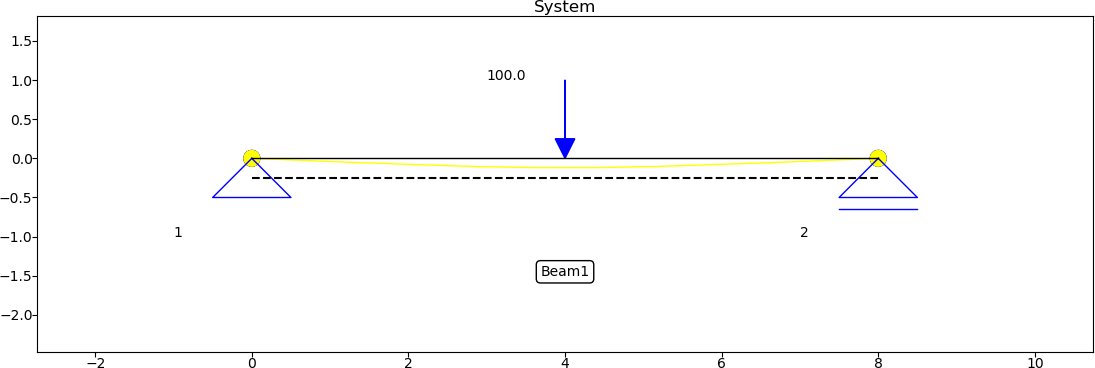
\includegraphics[width=0.9\textwidth]{example1/Figure_1.png}%
    \caption{Example 1: Single-Span Beam}%
    \label{fig:example1}%
\end{figure}

The visualization shows the advantage of using B\'{e}zier curves as a qualitative approximation for the deflection plot.
But it also becomes clear that there is still an error in the calculations since the strut end forces $S_l$ are wrong, there should be no torque but only lateral forces present.
At this point, I was unable to trace the error 

\section{Problems}
\label{sec:problems}

\subsection{Calculating $S_l$}
\label{sec:calc_Sl}

\subsection{Calculating Reactions}
\label{sec:calc_reactions}

\subsection{Second Order Analysis}
\label{sec:secondOrderAna}